% Asset ID: AS1ExponentialsAndLogarithmsTikZ-001
% Asset type: TikZ diagram
% Suggested file path: tikz/AS1ExponentialsAndLogarithmsTikZ-001.tex
% Unit code: AS1
% Topic code: AS1-EXPLOG
% Topic name: Exponentials and logarithms
% Related lesson section: Core Theory 3 and 4; Worked Example 2
% Source: Chapter 14 PDF and transcript; CCEA AS1-EXPLOG graph-sketching boundary
% Purpose: Show exponential growth and decay using y = 2^x and y = 2^{-x}.
\documentclass[tikz,border=8pt]{standalone}
\usepackage{amsmath}
\usepackage{pgfplots}
\pgfplotsset{compat=1.18}
\begin{document}
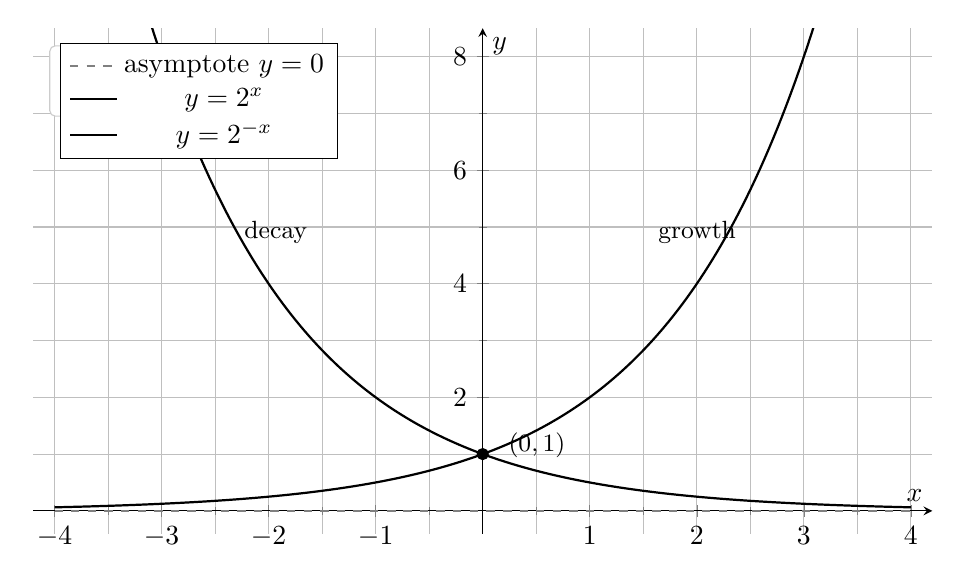
\begin{tikzpicture}
\begin{axis}[width=13cm,height=8cm,axis lines=middle,xmin=-4.2,xmax=4.2,ymin=-0.4,ymax=8.5,xlabel={$x$},ylabel={$y$},grid=both,minor tick num=1,samples=200,domain=-4:4,legend pos=north west]
\addplot[dashed,thick,gray]{0};\addlegendentry{asymptote $y=0$}
\addplot[thick]{2^x};\addlegendentry{$y=2^x$}
\addplot[thick]{2^(-x)};\addlegendentry{$y=2^{-x}$}
\addplot[only marks,mark=*,mark size=2pt] coordinates {(0,1)};
\node[anchor=west,font=\small] at (axis cs:0.15,1.15) {$(0,1)$};
\node[anchor=west,font=\small] at (axis cs:1.55,4.9) {growth};
\node[anchor=east,font=\small] at (axis cs:-1.55,4.9) {decay};
\node[align=left,anchor=north west,font=\small,fill=white,draw=black!20,rounded corners=2pt] at (axis cs:-4.05,8.2) {$2^{-x}=\left(\frac12\right)^x$\\Reflection in $x=0$.};
\end{axis}
\end{tikzpicture}
\end{document}
